%==========================オプションおよび文書クラスの設定==========================
%"autodetect-engine"-どのエンジンでもコンパイル可能にするオプション
%"dvipdfmx-if-dvi"-必要な場合のみdvipdfmx経由のpdf化をするオプション(LuaTeXやXeTeXはPDFに直接変換するため)
%"ja=standard"-日本語文書の標準設定を利用するオプション
%"bxjs…"-どのエンジンでも利用可能なドキュメントクラス
%--以下のいずれかを選択--
\documentclass[autodetect-engine,dvipdfmx-if-dvi,ja=standard,a4paper,11pt]{bxjsarticle} %章の無いレポート
%\documentclass[autodetect-engine,dvipdfmx-if-dvi,ja=standard,a4paper,10pt]{bxjsslide} %スライド
%\documentclass[autodetect-engine,dvipdfmx-if-dvi,ja=standard,a4paper,10pt]{bxjsbook} %書籍
%\documentclass[autodetect-engine,dvipdfmx-if-dvi,ja=standard,a4paper,10pt]{bxjsreport} %章のある論文やレポート

%==============================プリアンブルの設定==============================
\title{基礎勉強会第7回(多分)P47$\sim$P54} %タイトル
\author{新B4 福田真悟} %著者名
\date{2020.3.3}%日付 %日付下の余白をN[mm]減らす

%///////////////////////////////////////////////////////////////////////////////////////////////////////////
%////////////////////////////////////パッケージの読込み及び設定の書換え//////////////////////////////////////
%///////////////////////////////////////////////////////////////////////////////////////////////////////////
\usepackage{graphicx} %図の挿入に関するパッケージ
\usepackage{float} %[H]で図の位置を固定する機能をONにするパッケージ
\usepackage{subcaption} %サブキャプションに関するパッケージ
\captionsetup{labelsep=space} %サブキャプション後の":"を非表示にする
\usepackage{enumerate} %{enumerate}[]の,[]の中の通りの箇条書きにすることができるパッケージ
\usepackage{amsmath} %数式に関するパッケージ
\usepackage{mathtools} %数式に関するパッケージ
\usepackage{bm} %ベクトル表示のコマンドを追加するパッケージ
\usepackage{comment} %複数行のコメントアウトを可能にするパッケージ
\usepackage{ascmac} %枠に関するパッケージ
\usepackage{tabularx} %表に関するパッケージ
\setpagelayout{top=10truemm,bottom=15truemm,left=15truemm,right=15truemm}  %余白に関する設定の書換え(bxjs…クラスではgeometryパッケージは使用不可)
\graphicspath{{../figures/}} %図を挿入する際に.texファイルの上の階層にあるfiguresというフォルダを参照可能にする
\usepackage{url}

%余白に関する設定の書換え(bxjs…クラスではgeometryパッケージは使用不可)
\belowcaptionskip=-0pt %キャプション下の余白をN[pt]減らす
\graphicspath{{../figures/}} %図を挿入する際に.texファイルの上の階層にあるfiguresというフォルダを参照可能にする

%使用記号の追加
\newcommand{\divergence}{\mathrm{div}\,}  %ダイバー
\newcommand{\grad}{\mathrm{grad}\,}  %グラディエント
\newcommand{\rot}{\mathrm{rot}\,}  %ローテーション

%\pagestyle{myheadings} %myheading文字列 emptyページ番号なし plainフッダーに
%\markright{\footnotesize 2月28日(金)15:00~ 顔合わせ}%全ページ共通への挿入
%================================以下本文================================
\begin{document}
\maketitle %設定したタイトルの挿入
\setcounter{section}{1}
\setcounter{section}{2}
\section{多次元の確率分布}%sectionの前に*をつけると数字の振り分けが消える不思議
\subsection{2次元の確率分布}
\subsubsection{同時確率分布}
 2つの確率変数$X,Y$を定義する.この2つの変数が離散型で$X=x_i,Y=y_j$となる確率は,
\begin{equation}
P(X=x_i,Y=y_j)=f(x_i,y_j)
\end{equation}
となる.これを同時確率分布という.連続型のときは,確率を範囲で考えるので$(x,y),(x+{\Delta}x,y),(x,y+{\Delta}y),(x+{\Delta}x,y+{\Delta}y)$の4点で囲まれた長方形に入る確率を考えるので,
\begin{equation}
f(x,y)=\frac{P(x<X\leq x+{\Delta}x,y<Y\leq y+{\Delta}y)}{{\Delta}x{\Delta}y} 
\end{equation}
${\Delta}x\rightarrow0,{\Delta}y\rightarrow0$と極限をとったときの$f(x,y)$を同時確率密度関数という.
 2変数における累積分布関数は,連続型と離散型でそれぞれ,
\begin{eqnarray}
F(x,y)=P(X\leq x,Y\leq y)=\left\{ \begin{array}{ll}
\displaystyle\sum_{u\leq x}\sum_{v\leq y}f(u,v) &  (\mbox{離散型}) \\
\displaystyle\int_{-\infty}^{x}\int_{-\infty}^{y}f(u,v)dudv & (\mbox{連続型}) \\
\end{array} \right.
\end{eqnarray}
となる.これを同時分布関数または,同時累積分布関数という.


\subsubsection{共分散と相関係数}
 2つの確率分布が存在する場合に知りたい情報として,その2つの情報の関係性がある.そのときに関係性を表す指標として,共分散と相関係数が用いられる.まず共分散は,
\begin{equation}
\label{eq:xyvar}
{\rm cov}(X,Y)=\sigma_{XY}=E[(X-\mu_X)(Y-\mu_Y)] 
\end{equation}
で書かれる.また,2変数のときの期待値演算子$E$は,
\begin{eqnarray}
E[\varphi(X,Y)] =\left\{ \begin{array}{ll}
\displaystyle\sum_{x}\sum_{y}\varphi(x,y)f(x,y) &  (\mbox{離散型}) \\
\displaystyle\int_{-\infty}^{\infty}\int_{-\infty}^{\infty}\varphi(x,y)f(x,y)dxdy & (\mbox{連続型}) \\
\end{array} \right.
\end{eqnarray}
となる.よって,式(\ref{eq:xyvar})は,
\begin{eqnarray}
\sigma_{XY}=\left\{ \begin{array}{ll}
\displaystyle\sum_{x}\sum_{y}(x-\mu_X)(y-\mu_Y)f(x,y) &  (\mbox{離散型}) \\
\displaystyle\int_{-\infty}^{\infty}\int_{-\infty}^{\infty}(x-\mu_X)(y-\mu_Y)f(x,y)dxdy & (\mbox{連続型}) \\
\end{array} \right.
\end{eqnarray}
となる.
 相関係数は,共分散を$X,Y$の個々のばらつき(分散)に依存しない(スケール不変性)で2変数の関係性のみを評価するために基準化を行ったものである.式は,
\begin{equation}
\rho=\frac{\sigma_{XY}}{\sigma_{X}\sigma_{Y}}
\end{equation}
となる.個々の確率変数のスケールを$X=aU+b,Y=cV+d$と変えたとき,共分散と各標準偏差は,
\begin{equation}
\sigma_{UV}=ac\sigma_{XY}
\end{equation}
\begin{equation}
\sigma_{U}=a\sigma_{X}
\end{equation}
\begin{equation}
\sigma_{V}=c\sigma_{Y}
\end{equation}
となる.よってスケールを$U,V$に変えたときの相関係数は,
\begin{equation}
\rho=\frac{ac\sigma_{XY}}{a\sigma_{X}c\sigma_{Y}}=\frac{\sigma_{XY}}{\sigma_{X}\sigma_{Y}}
\end{equation}
となり,スケールを変えても相関係数は変化しないことがわかる.具体的にイメージするために確率変数$X,Y$の条件のもと,試行を$N$回繰り返したときの$i$回目の試行の結果を$(x_i,y_i)$とする.ここでの$N$は十分に大きい整数とする.$X,Y$の結果とそれぞれの平均値との差のベクトル${\bf X}=(x_1-\mu_X,x_2-\mu_X,\cdots,x_N-\mu_X),{\bf Y}=(y_1-\mu_Y,y_2-\mu_Y,\cdots,y_N-\mu_Y)$としたとき,$\sigma_{XY}$は,大数の法則弱より,内積${\bf X\cdot Y}$を回数$N$で除したものとなる.$\sigma_{X}^2,\sigma_{Y}^2$は,それぞれ${\bf |X|^2,|Y|^2}$を回数$N$で除したものとなる.このとき,相対係数$\rho$は,
\begin{equation}
\rho=\frac{X\cdot Y}{|X||Y|}
\end{equation}
となる.ベクトルで考えたとき,二つのベクトル${\bf X},{\bf Y}$のなす角度を$\theta$とおいたとき,相対係数は,内積の公式から,
\begin{equation}
\rho=\cos{\theta}
\end{equation}
となることがわかる.このため範囲が$-1\leq\rho\leq1$となる.また,このことから相関係数が示しているのはベクトルのなす角度であり,相関係数はあくまで線形の関係の${\bf Y}=A{\bf X}+B$があるかどうかを示していることがわかる.また,相対係数の結果を比較を行うとき$\cos{\theta}$のため,大小の比較しか行えないことがわかる.


\subsubsection{周辺確率分布,条件付確率分布および独立}
\setlength{\leftmargini}{0pt}
\begin{itemize}
\item 周辺確率\\
 $X$と$Y$の個々の確率分布を周辺確率分布という.それぞれ離散型と連続型は,
 \begin{eqnarray}
 g(x)=\left\{ \begin{array}{ll}
 \displaystyle\sum_{y}f(x,y) &  (\mbox{離散型}) \\
 \displaystyle\int_{-\infty}^{\infty}f(x,y)dy & (\mbox{連続型}) \\
 \end{array} \right.
 \end{eqnarray}
 \begin{eqnarray}
h(y)=\left\{ \begin{array}{ll}
\displaystyle\sum_{x}f(x,y) &  (\mbox{離散型}) \\
\displaystyle\int_{-\infty}^{\infty}f(x,y)dx & (\mbox{連続型}) \\
\end{array} \right.
\end{eqnarray}
となる.
 
\item 条件付確率\\
 条件付確率は,
\begin{equation}
P(X=x|Y=y)=\frac{P(X=x,Y=y)}{P(Y=y)}
\end{equation}
となる.周辺確率と合わせると,
\begin{equation}
g(x|y)=P(X=x|Y=y)=\frac{f(x,y)}{h(y)}
\end{equation}
となる.これは連続型でも拡張ができ,条件付確率密度関数という.また,条件付確率も総和は1となる条件を満足する.条件付確率の期待値,分散は,それぞれの確率密度関数を$f(x,y)$から$g(x|y)$などに変えることで導出できる.

\item 独立\\
 独立のときは,条件付確率がそれぞれ,
\begin{equation}
g(x|y)=g(x),h(y|x)=h(y)
\end{equation}
となる.この式から,
\begin{equation}
f(x,y)=g(x)h(y)
\end{equation}
となる.上記の式と$X,Y$が独立であることは必要十分条件である.

\item 独立の場合の相関係数\\
\begin{equation}
\begin{split}
{\rm cov}(X,Y)&=\displaystyle\int_{-\infty}^{\infty}\int_{-\infty}^{\infty}(x-\mu_X)(y-\mu_Y)f(x,y)dxdy\\
&=\displaystyle\int_{-\infty}^{\infty}\int_{-\infty}^{\infty}(x-\mu_X)(y-\mu_Y)g(x)h(y)dxdy\\
&=\displaystyle\int_{-\infty}^{\infty}(x-\mu_X)g(x)dx\int_{-\infty}^{\infty}(y-\mu_Y)h(y)dy\\
&=0
\end{split}
\end{equation}
となるため,相関係数は0となる.相関係数が0のとき,$X,Y$が独立になるわけではない.反例として,$Y=X^2$の相関がある場合が挙げられる.独立の場合,
\begin{equation}
E[\varphi(X)\psi(Y)]=E[\varphi(X)]E[\psi(Y)]
\end{equation}
が成り立つ.
\end{itemize}






\subsubsection{確率変数の和の分布と期待値と分散}
\begin{itemize}
\item 確率変数の和の分布\\
 $Z$を2つの確率変数$X,Y$の和$Z=X+Y$としたときの$Z$の確率密度関数は,
\begin{eqnarray}
\label{wonoiki}
k(z)=\left\{ \begin{array}{ll}
\displaystyle\sum_{x}f(x,z-x) &  (\mbox{離散型}) \\
\displaystyle\int_{-\infty}^{\infty}f(x,z-x)dx & (\mbox{連続型}) \\
\end{array} \right.
\end{eqnarray}
となる.特に$X,Y$が独立の場合は,
\begin{eqnarray}
k(z)=\left\{ \begin{array}{ll}
\displaystyle\sum_{x}g(x)h(z-x) &  (\mbox{離散型}) \\
\displaystyle\int_{-\infty}^{\infty}g(x)h(z-x)dx & (\mbox{連続型}) \\
\end{array} \right.
\end{eqnarray}
となり,これをたたみこみといい,$k=g*h$で表現される.

\item 再生性\\
  一般的に確率変数の和の分布を導出するには,式(\ref{wonoiki})を用いるが,一部の分布においては独立な確率変数の和は同一の分布形になるものがある.このような分布を再生的という.二項分布,ポアソン分布,負の二項分布,正規分布,ガンマ分布などがある.各分布に関しての再現性について下記に記載する.\\
  まず二項分布について.$X\sim Bi(n_1,P),Y\sim Bi(n_2,P)\Rightarrow Z=X+Y\sim Bi(n_1+n_2,P)$となる.$X,Y,Z$のそれぞれは,
\begin{equation}
g(x)={}_{n_1} C_xP^x(1-P)^{n_1-x}
\end{equation}
\begin{equation}
h(z-x)={}_{n_2} C_{z-x}P^{z-x}(1-P)^{n_2-(z-x)}
\end{equation}
\begin{equation}
\label{Bi_z}
k(z)=\displaystyle\sum_{x}{}_{n_1} C_x\cdot{}_{n_2} C_{z-x}P^z(1-P)^{n_1+n_2-z}
\end{equation}
となる.ここで
\begin{equation}
{}_{n_1+n_2} C_z=\displaystyle\sum_{x}{}_{n_1} C_x\cdot{}_{n_2} C_{z-x}
\end{equation} 
となるので,式(\ref{Bi_z})に代入すると,
\begin{equation}
k(z)={}_{n_1+n_2} C_zP^z(1-P)^{n_1+n_2-z}=Bi(n_1+n_2,P)
\end{equation}
となる.また,負の二項分布も同様である.\\
 次にポアソン分布について.$X\sim Po(\lambda_1),Y\sim Po(\lambda_2)\Rightarrow Z=X+Y\sim Po(\lambda_1+\lambda_2)$となる.$X,Y,Z$のそれぞれは,
\begin{equation}
g(x)=\frac{\mathrm{e}^{-\lambda_1}\lambda_1^x}{x!}
\end{equation}
\begin{equation}
h(z-x)=\frac{\mathrm{e}^{-\lambda_2}\lambda_2^{z-x}}{(z-x)!}
\end{equation}
\begin{equation}
\label{Po_z}
k(z)=\displaystyle\sum_{x}\frac{\mathrm{e}^{-(\lambda_1+\lambda_2)}\lambda_1^x\lambda_2^{z-x}}{x!(z-x)!}
\end{equation}
となる.ここで${}_{z} C_x=\frac{z!}{x!(z-x)!}$を用いると式(\ref{Po_z})は,
\begin{equation}
k(z)=\frac{\mathrm{e}^{-(\lambda_1+\lambda_2)}}{z!}\displaystyle\sum_{x}{}_{z} C_x\lambda_1^x\lambda_2^{z-x}
\end{equation} 
となり,二項定理から,
\begin{equation} 
\displaystyle\sum_{x}{}_{z} C_x\lambda_1^x\lambda_2^{z-x}=(\lambda_1+\lambda_2)^z
\end{equation}
となるので代入すると,
\begin{equation}
k(z)=\frac{\mathrm{e}^{-(\lambda_1+\lambda_2)}(\lambda_1+\lambda_2)^z}{z!}=Po(\lambda_1+\lambda_2)
\end{equation}
となる.\\
 次に正規分布について.$X\sim N(\mu_1,\sigma_1^2),Y\sim N(\mu_2,\sigma_2^2)\Rightarrow Z=X+Y\sim N(\mu_1+\mu_2,\sigma_1^2+\sigma_2^2)$となる.$X,Y,Z$のそれぞれは,
\begin{equation}
g(x)=\frac{1}{\sqrt{2\pi}\sigma_1}{\rm exp}\left[\frac{-(x-\mu_1)^2}{2\sigma_1^2}\right]
\end{equation}
\begin{equation}
g(z-x)=\frac{1}{\sqrt{2\pi}\sigma_2}{\rm exp}\left[\frac{-((z-x)-\mu_2)^2}{2\sigma_2^2}\right]
\end{equation}
\begin{equation}
\label{N_z}
k(z)=\displaystyle\int_{-\infty}^{\infty}\frac{1}{2\pi\sigma_1\sigma_2}{\rm exp}\left[\frac{-(x-\mu_1)^2}{2\sigma_1^2}+\frac{-((z-x)-\mu_2)^2}{2\sigma_2^2}\right]dx
\end{equation}
となる.ガウス積分などを用いて計算を行うと,
\begin{equation}
g(x)=\frac{1}{\sqrt{2\pi}\sqrt{\sigma_1^2+\sigma_2^2}}{\rm exp}\left[\frac{-(z-(\mu_1+\mu_2))^2}{2(\sigma_1^2+\sigma_2^2)}\right]=N(\mu_1+\mu_2,\sigma_1^2+\sigma_2^2)
\end{equation} 
となる.\\
 最後にガンマ分布について.$X\sim Ga(\alpha_1,\beta),Y\sim Ga(\alpha_2,\beta)\Rightarrow Z=X+Y\sim Ga(\alpha_1+\alpha_2,\beta)$となる.$X,Y,Z$のそれぞれは,
\begin{equation}
g(x)=\frac{1}{\beta^{\alpha_1}\Gamma(\alpha_1)}x^{\alpha_1-1}\mathrm{e}^{-\frac{x}{\beta}}
\end{equation}
\begin{equation}
h(z-x)=\frac{1}{\beta^{\alpha_2}\Gamma(\alpha_2)}(z-x)^{\alpha_2-1}\mathrm{e}^{-\frac{z-x}{\beta}}
\end{equation}
\begin{equation}
\label{Ga_z}
k(z)=\frac{1}{\beta^{\alpha_1+\alpha_2}\Gamma(\alpha_1)\Gamma(\alpha_2)}\mathrm{e}^{-\frac{z}{\beta}}\displaystyle\int_{0}^{z}x^{\alpha_1-1}(z-x)^{\alpha_2-1}dx
\end{equation}
となる.積分区間については,ガンマ分布が$x<0$の範囲では$0$となるので,[0,z]の区間になっている.ここでベータ関数$B(\alpha_1,\alpha_2)$を導入すると,
\begin{equation}
B(\alpha_1,\alpha_2)=\displaystyle\int_{0}^{1}t^{\alpha_1-1}(1-t)^{\alpha_2-1}dt
\end{equation} 
となる.ここで$t=x/z$($z$は定数,$x$は変数)で置換すると,
\begin{equation}
B(\alpha_1,\alpha_2)=\displaystyle\int_{0}^{z}z^{-(\alpha_1-1)}x^{\alpha_1-1}z^{-(\alpha_2-1)}(z-x)^{\alpha_2-1}z^{-1}dx
\end{equation}
となる.まとめると,
\begin{equation}
B(\alpha_1,\alpha_2)=\frac{1}{z^{\alpha_1+\alpha_2-1}}\displaystyle\int_{0}^{z}x^{\alpha_1-1}(z-x)^{\alpha_2-1}dx
\end{equation}
となる.さらにベータ関数とガンマ関数の間には下記の等式が成り立つ.
\begin{equation}
\label{B_Ga}
B(\alpha_1,\alpha_2)=\frac{\Gamma(\alpha_1)\Gamma(\alpha_2)}{\Gamma(\alpha_1+\alpha_2)}=\frac{1}{z^{\alpha_1+\alpha_2-1}}\displaystyle\int_{0}^{z}x^{\alpha_1-1}(z-x)^{\alpha_2-1}dx
\end{equation}
となる.式(\ref{B_Ga})を式(\ref{Ga_z})に代入すると,
\begin{equation}
k(z)=\frac{1}{\beta^{\alpha_1+\alpha_2}\Gamma(\alpha_1+\alpha_2)}z^{\alpha_1+\alpha_2-1}\mathrm{e}^{-\frac{z}{\beta}}=Ga(\alpha_1+\alpha_2,\beta)
\end{equation}


\item 確率変数の和の期待値と分散\\
確率変数の和の期待値は,
\begin{equation}
E(Z)=E(X+Y)=\displaystyle\int_{-\infty}^{\infty}\int_{-\infty}^{\infty}(x+y)f(x,y)dxdy=E(X)+E(Y)=\mu_X+\mu_Y
\end{equation}
となり,期待値も$X,Y$の和となる.一方で分散は,
\begin{equation}
\begin{split}
V(X+Y)&=E[\{(X+Y)-(\mu_X+\mu_Y)\}^2]\\
&=E[(X-\mu_X)^2]+E[(Y-\mu_Y)^2]+2E[(X-\mu_X)(Y-\mu_Y)]\\
&=V(X)+V(Y)+2{\rm cov}(X,Y)\\
&=\sigma_X^2+\sigma_Y^2+2\sigma_{XY}\\
\end{split}
\end{equation}
となり,ただの和にはならないので注意が必要である.
\end{itemize}


%\begin{figure}[H]%[h]は記述したところ。[t]はそのページの上端。[t]はそのページの下端、[p]はページいっぱい
%\begin{center}
%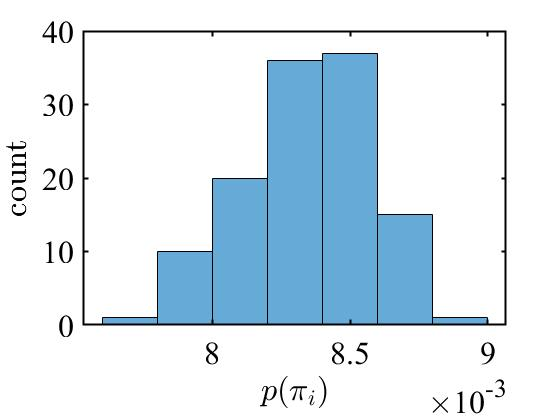
\includegraphics[width=.4\textwidth]{kadai3_histo.jpg}
%\end{center}
%\caption{課題3のヒストグラム(生成数は$100000$)}%図名
%\label{fig:kadai3_3}
%\end{figure}

%チェビシェフの不等式の置き換えの大数の弱法則から,
%\begin{equation}
%P(|\overline{X}_n-\mu|\ge \epsilon) \le \dfrac{\sigma^2}{n \epsilon^2}
%\end{equation}
%となる.ここでの$\overline{X}_n$はサンプルデータ$n$までの平均値(標本),$\mu$は理論的に考えられる平均値,$\epsilon$は許容誤差の大きさ,$\sigma$は標本データの分散である.




%$A^1$\cite{aaa}%参考文献




%\begin{itemize}
%\item アイテムコード1\\
%\item アイテムコード2\\
%\item アイテムコード3\\
%\item アイテムコード4\\
%\item アイテムコード5\\
%\end{itemize}


%\begin{figure}[H]%[h]は記述したところ。[t]はそのページの上端。[t]はそのページの下端、[p]はページいっぱい
%\begin{center}
%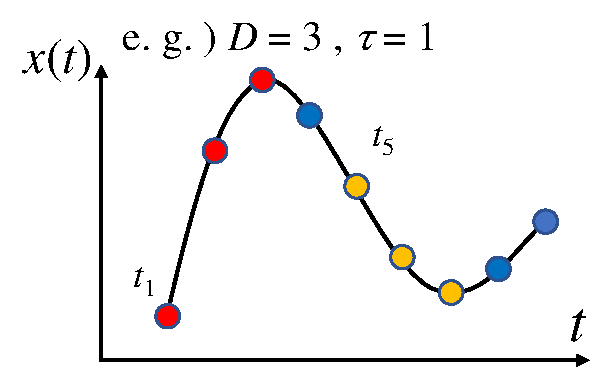
\includegraphics[width=.4\textwidth]{crop_PE1ver2.pdf} 
%\end{center}
%\caption{時系列$ x(t) $}%図名
%\label{fig:PE1}%fig図tb表
%\end{figure}

%\begin{eqnarray}
%\left\{%%{を作る
%\begin{array}{l}%l,llでは、lのときすべて{}の中の式のとき、{}の中にないものがあるならこっち
%\end{array}
%\right.
%\end{eqnarray} 


\begin{thebibliography}{9999}%参考文献
\bibitem{lo}%参考文献citeするぞ
東京大学工学教程基礎系数学確率統計Ⅰ,縄田和満,平成25年10月10日
%\bibitem{re}
%カオス・フラクタル\ 講義ノート\ \#8,\url{https://ocw.hokudai.ac.jp/wp-content/uploads/2016/01/ChaosFractal-2011-Note-08.pdf}
%\bibitem{wgn}%参考文献citeするぞ
%ホワイトガウスノイズサンプルの生成-MATLAD wgn,\url{https://jp.mathworks.com/help/comm/ref/wgn.html}
%\bibitem{mutual}
%相互情報量の意味とエントロピーとの関係 | 高校数学の美しい物語,\url{https://mathtrain.jp/mutualinfo}
%\bibitem{net}
%複雑ネットワーク:統計物理学の視点,\url{http://mercury.yukawa.kyoto-u.ac.jp/~bussei.kenkyu/pdf/03/1/9999-031210.pdf}
\end{thebibliography}

%\newpage



\end{document}